\chapter{Results}



%%%%%%%%%%%%%%%%%
%%             %%
%%   PSO2006   %%
%%             %%
%%%%%%%%%%%%%%%%%
\begin{figure}[ht!]
    \centering
    \begin{minipage}[t]{0.32\textwidth}
        \centering
        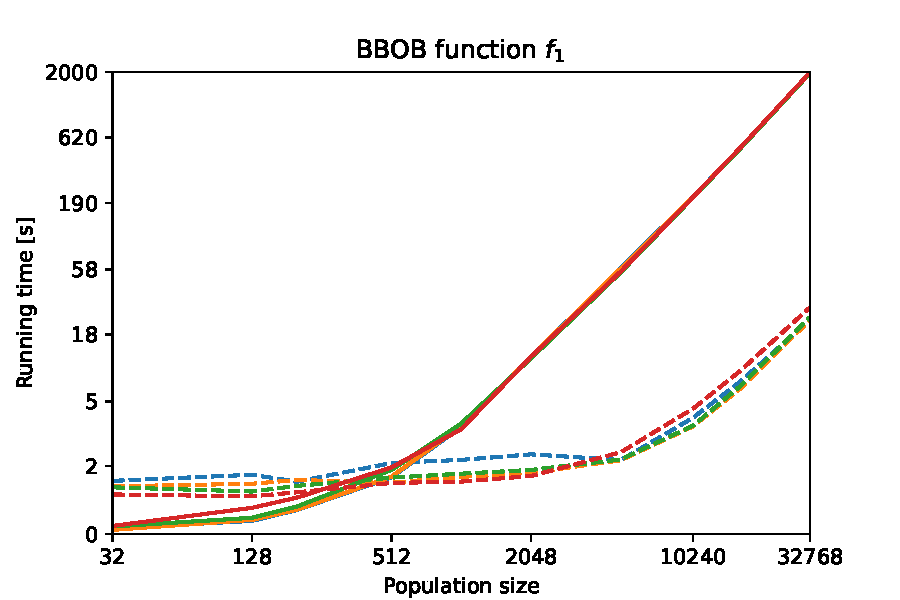
\includegraphics[width=\textwidth]{img/runs/time_pso2006_fn1_alldim.pdf}
    \end{minipage}
    \hfill
    \begin{minipage}[t]{0.32\textwidth}
        \centering
        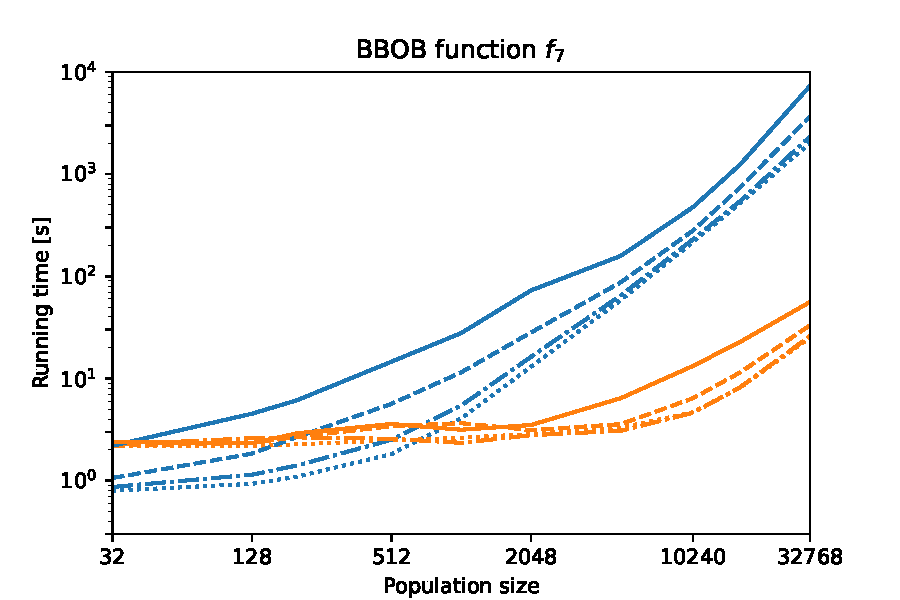
\includegraphics[width=\textwidth]{img/runs/time_pso2006_fn7_alldim.pdf}
    \end{minipage}
    \hfill
    \begin{minipage}[t]{0.32\textwidth}
        \centering
        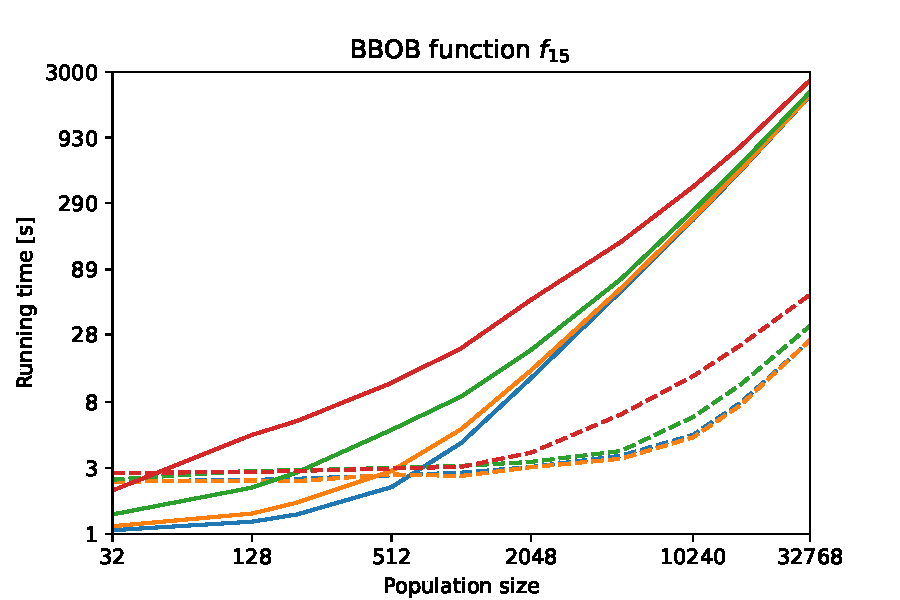
\includegraphics[width=\textwidth]{img/runs/time_pso2006_fn15_alldim.pdf}
    \end{minipage}

    \centering
    \begin{minipage}[t]{0.32\textwidth}
        \centering
        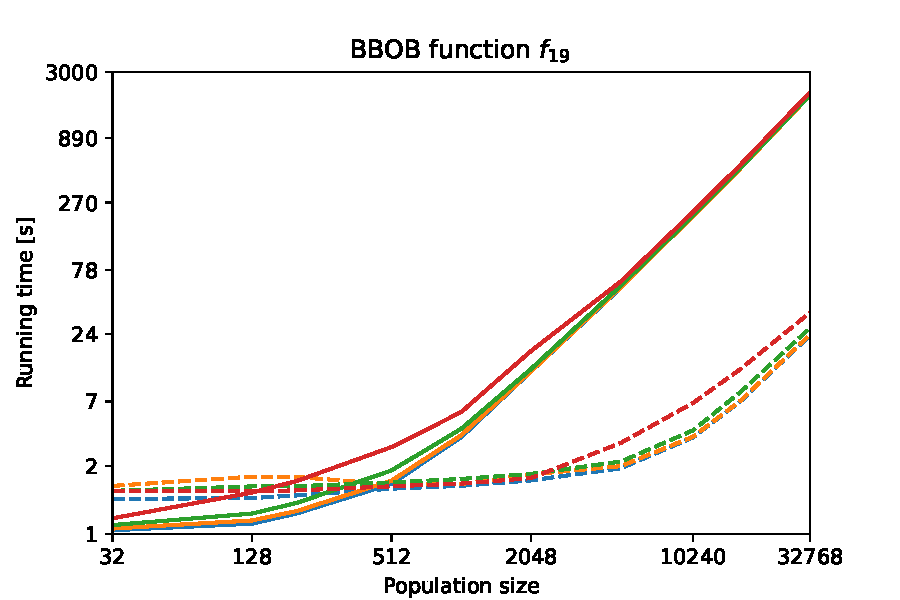
\includegraphics[width=\textwidth]{img/runs/time_pso2006_fn19_alldim.pdf}
    \end{minipage}
    \hfill
    \begin{minipage}[t]{0.32\textwidth}
        \centering
        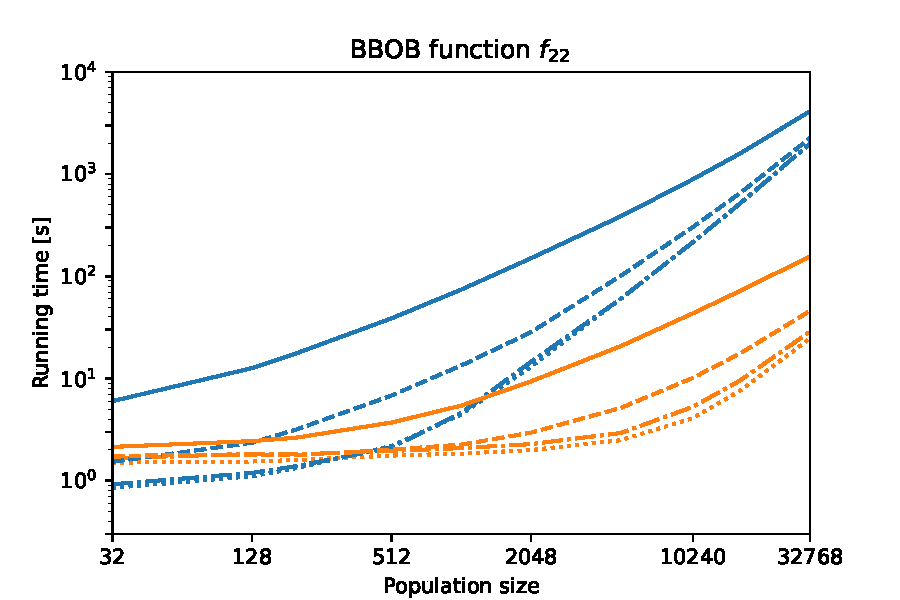
\includegraphics[width=\textwidth]{img/runs/time_pso2006_fn22_alldim.pdf}
    \end{minipage}
    \hfill
    \begin{minipage}[t]{0.32\textwidth}
        \centering
        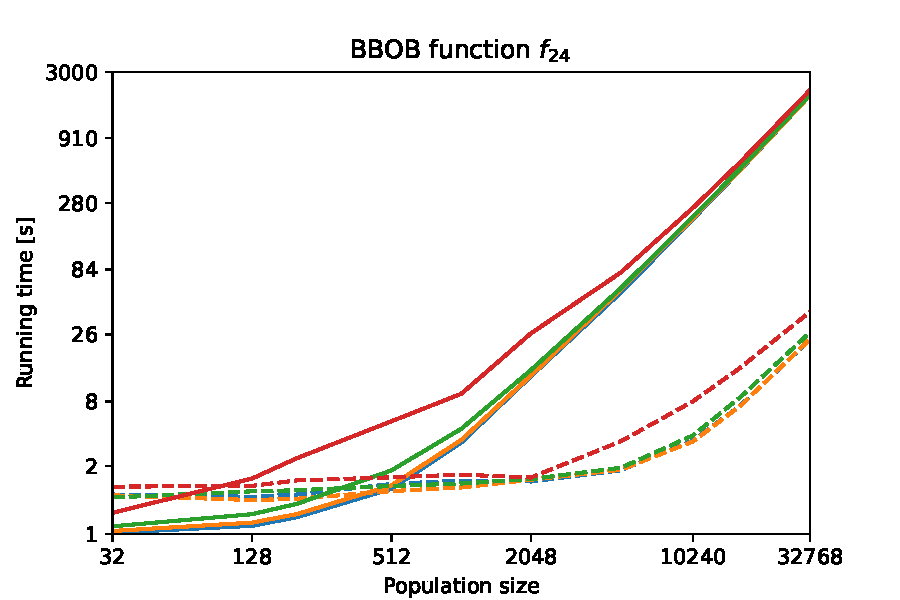
\includegraphics[width=\textwidth]{img/runs/time_pso2006_fn24_alldim.pdf}
    \end{minipage}

    \begin{minipage}{\textwidth}
        \centering
        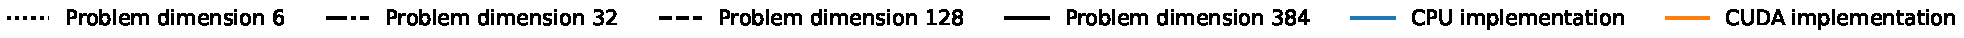
\includegraphics[width=\textwidth]{img/runs/time_pso2006_alldim_legend.pdf}
    \end{minipage}

    \caption[PSO2006 running times]{Running times of \acrlong{acc:spso2006} algorithm using problem of dimension $6$, $32$, $128$, and $384$. The algorithm run for $1000$ generations. Populations with over $1000$ particles takes advantage of \gpu.}
\end{figure}

\begin{figure}[ht!]
    \centering
    \begin{minipage}[t]{0.32\textwidth}
        \centering
        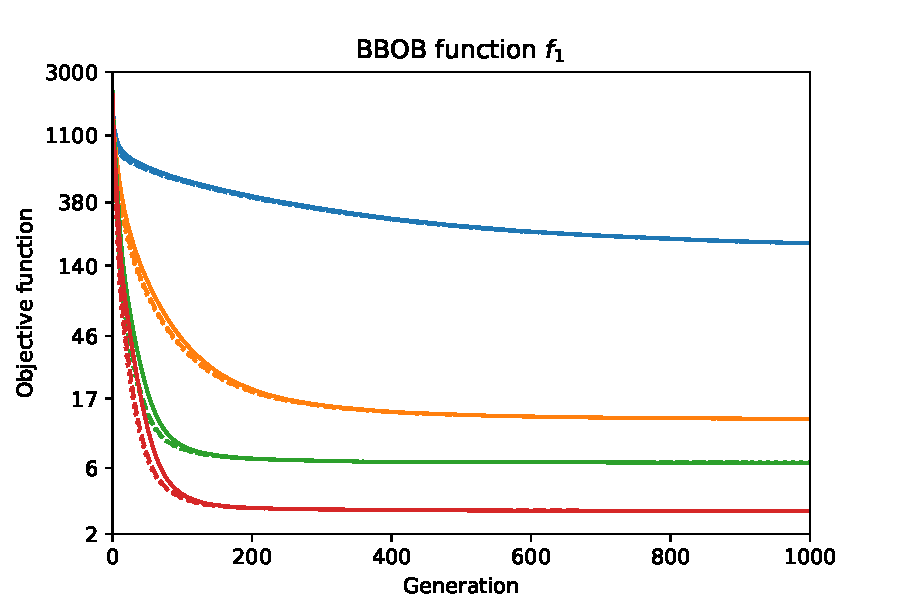
\includegraphics[width=\textwidth]{img/runs/fitness_pso2006_f1.pdf}
    \end{minipage}
    \hfill
    \begin{minipage}[t]{0.32\textwidth}
        \centering
        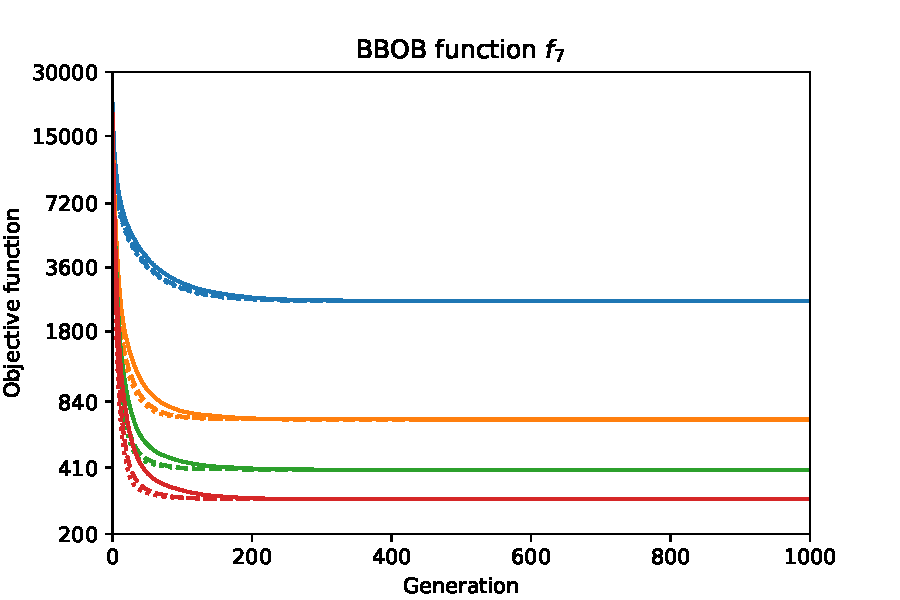
\includegraphics[width=\textwidth]{img/runs/fitness_pso2006_f7.pdf}
    \end{minipage}
    \hfill
    \begin{minipage}[t]{0.32\textwidth}
        \centering
        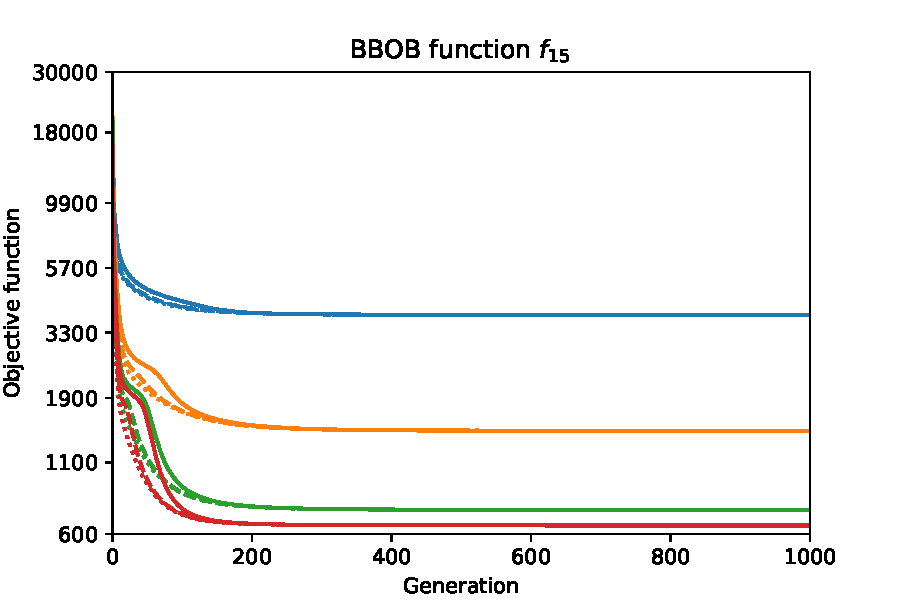
\includegraphics[width=\textwidth]{img/runs/fitness_pso2006_f15.pdf}
    \end{minipage}

    \centering
    \begin{minipage}[t]{0.32\textwidth}
        \centering
        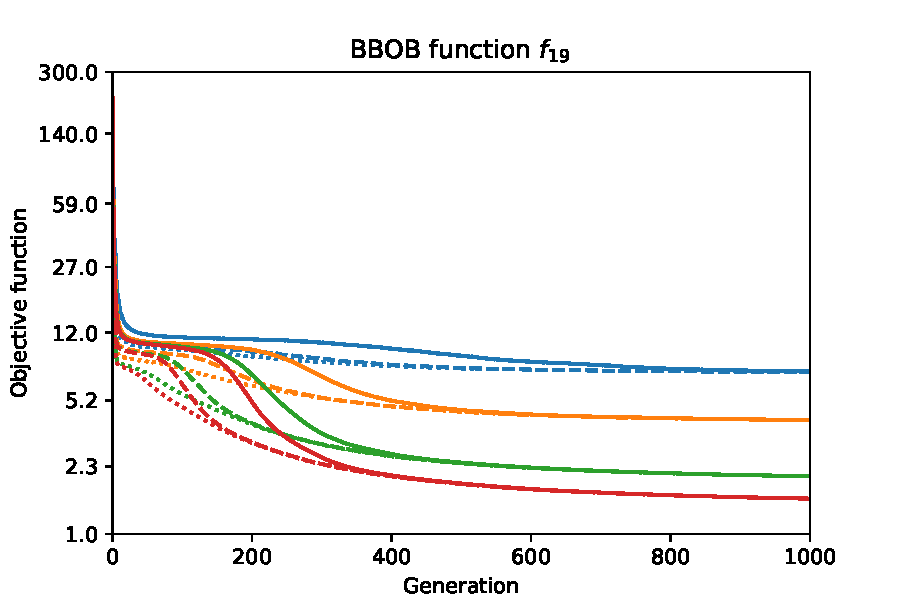
\includegraphics[width=\textwidth]{img/runs/fitness_pso2006_f19.pdf}
    \end{minipage}
    \hfill
    \begin{minipage}[t]{0.32\textwidth}
        \centering
        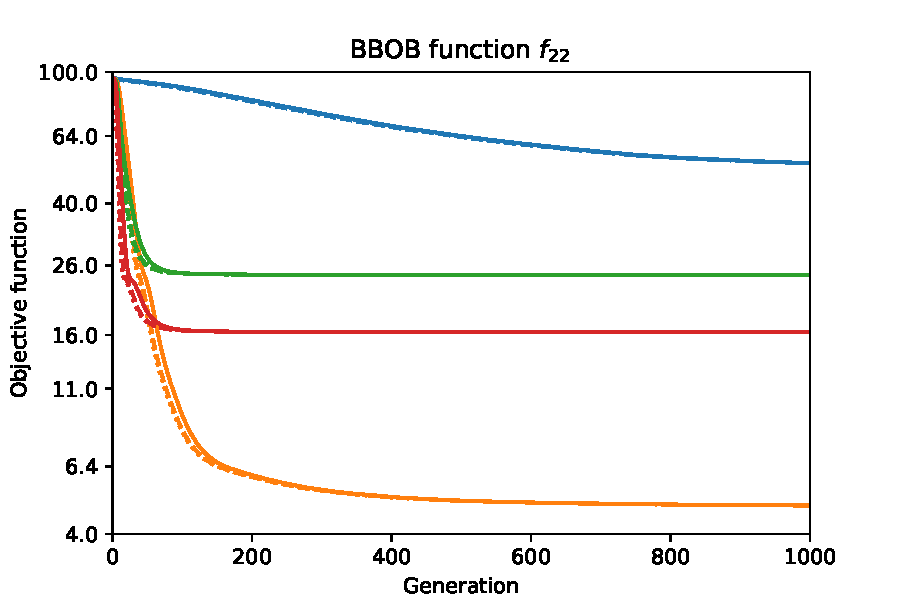
\includegraphics[width=\textwidth]{img/runs/fitness_pso2006_f22.pdf}
    \end{minipage}
    \hfill
    \begin{minipage}[t]{0.32\textwidth}
        \centering
        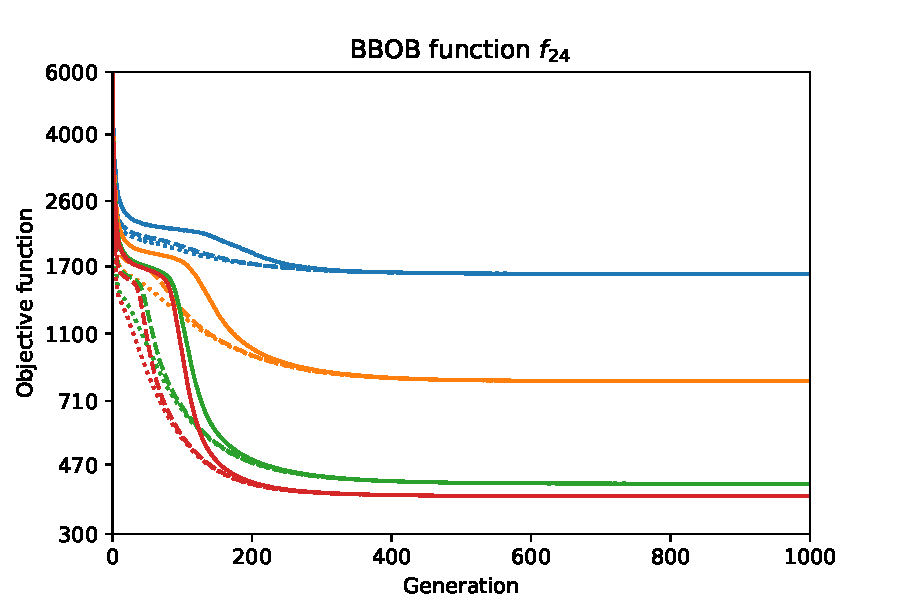
\includegraphics[width=\textwidth]{img/runs/fitness_pso2006_f24.pdf}
    \end{minipage}

    \begin{minipage}{\textwidth}
        \centering
        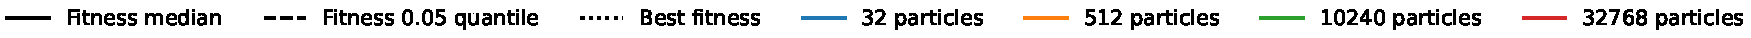
\includegraphics[width=\textwidth]{img/runs/fitness_pso2011_legend.pdf}
    \end{minipage}

    \caption[PSO2006 fitness over generations]{Median, $0.05$ quantile, and best fitness of \acrlong{acc:spso2006} algorithm using random neighborhood on problem of $128$ dimensions. I measured populations consisting of $32$, $512$, $10240$, and $32768$ particles. All the problem functions take advantage of more particles, except of function $f_7$. Given hyperparameters in table \ref{tab:psohyperparameters}, \acrshort{acc:spso2006} seems to have better convergence properties in comparison to \acrshort{acc:spso2011}.}
\end{figure}



%%%%%%%%%%%%%%%%%
%%             %%
%%   PSO2011   %%
%%             %%
%%%%%%%%%%%%%%%%%
\begin{figure}[ht!]
    \centering
    \begin{minipage}[t]{0.32\textwidth}
        \centering
        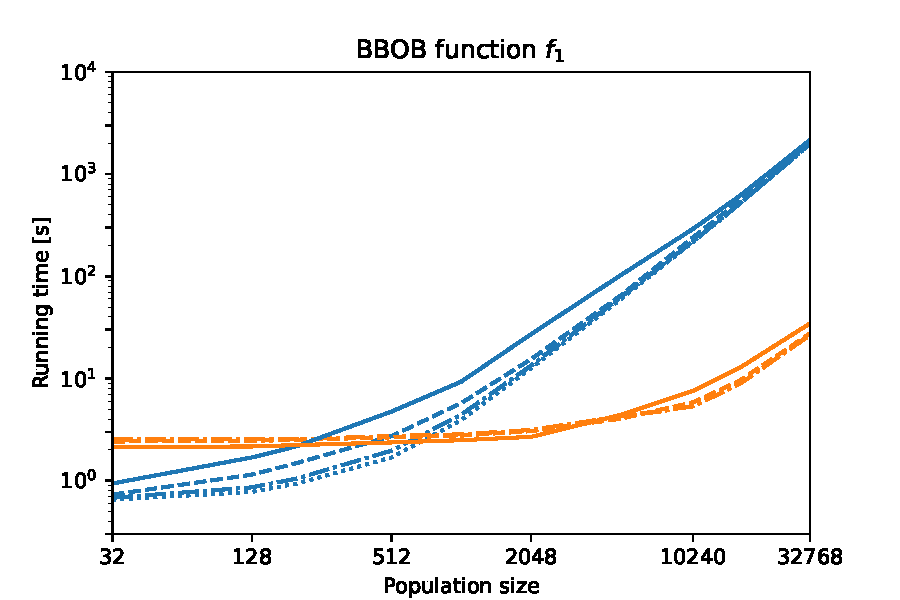
\includegraphics[width=\textwidth]{img/runs/time_pso2011_fn1_alldim.pdf}
    \end{minipage}
    \hfill
    \begin{minipage}[t]{0.32\textwidth}
        \centering
        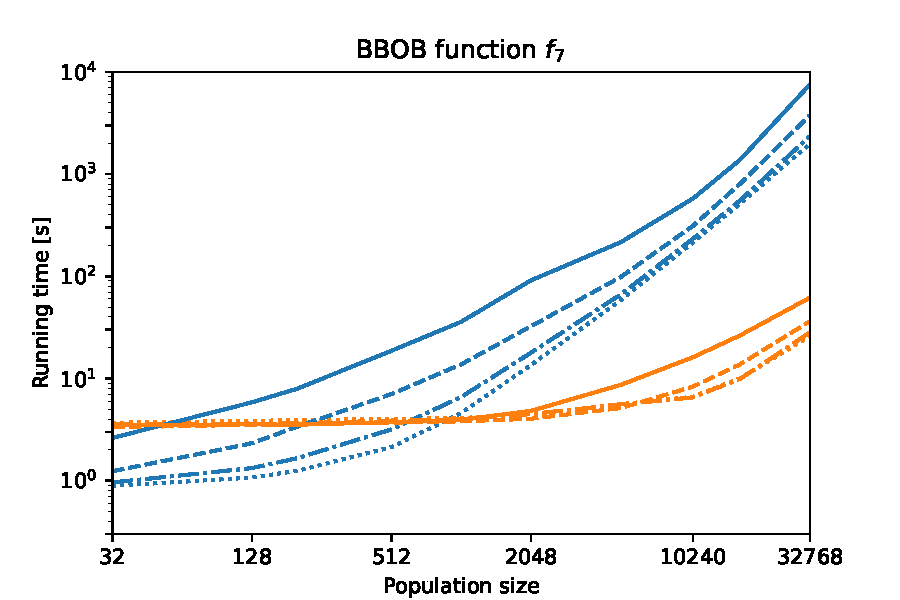
\includegraphics[width=\textwidth]{img/runs/time_pso2011_fn7_alldim.pdf}
    \end{minipage}
    \hfill
    \begin{minipage}[t]{0.32\textwidth}
        \centering
        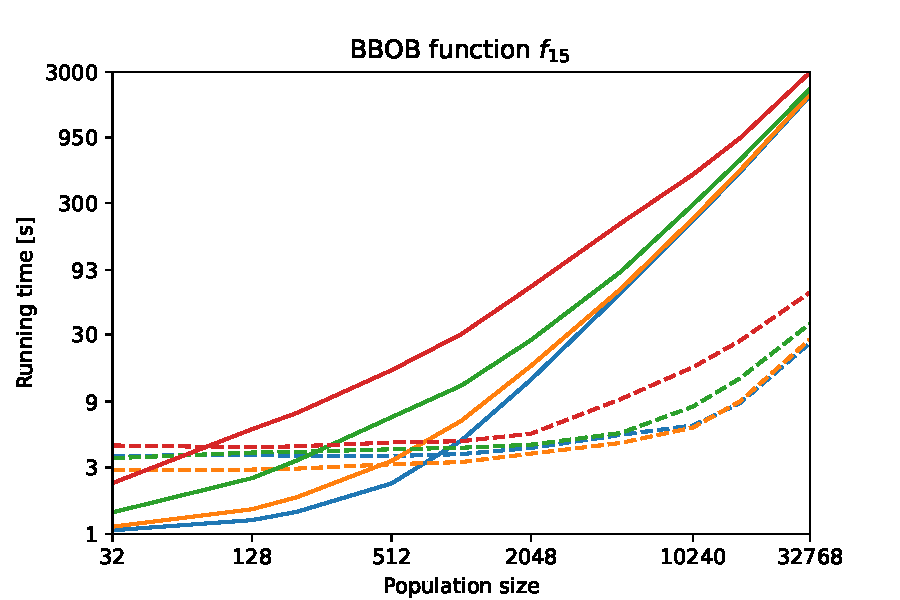
\includegraphics[width=\textwidth]{img/runs/time_pso2011_fn15_alldim.pdf}
    \end{minipage}

    \centering
    \begin{minipage}[t]{0.32\textwidth}
        \centering
        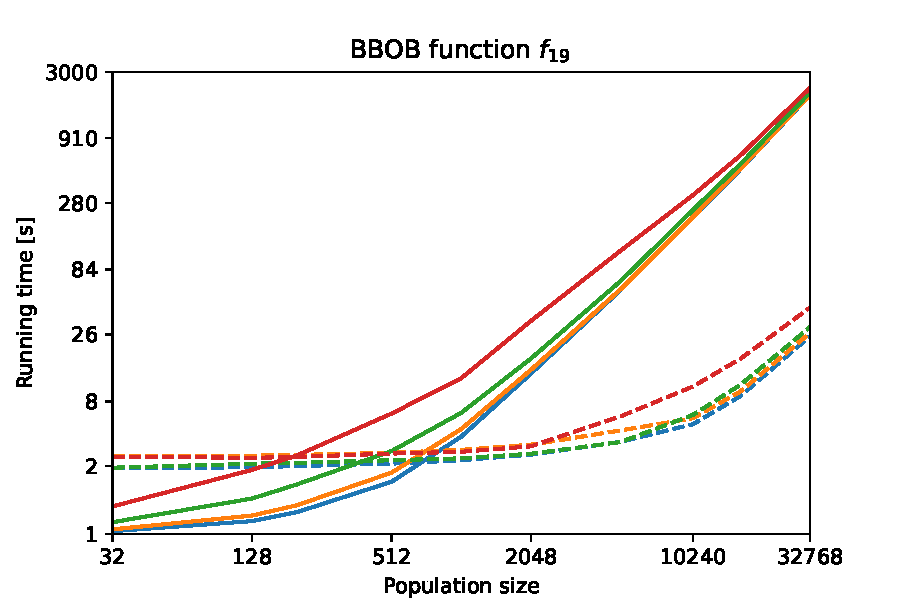
\includegraphics[width=\textwidth]{img/runs/time_pso2011_fn19_alldim.pdf}
    \end{minipage}
    \hfill
    \begin{minipage}[t]{0.32\textwidth}
        \centering
        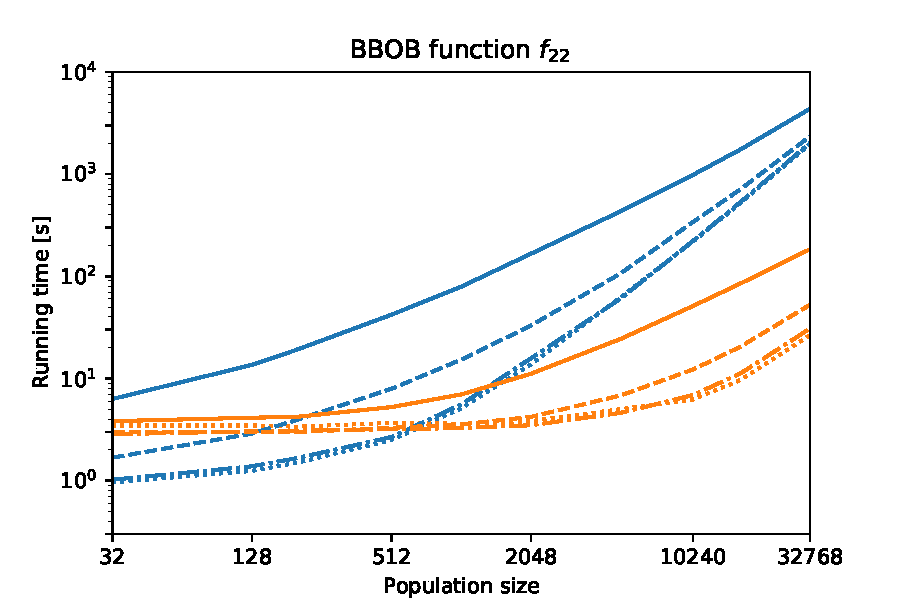
\includegraphics[width=\textwidth]{img/runs/time_pso2011_fn22_alldim.pdf}
    \end{minipage}
    \hfill
    \begin{minipage}[t]{0.32\textwidth}
        \centering
        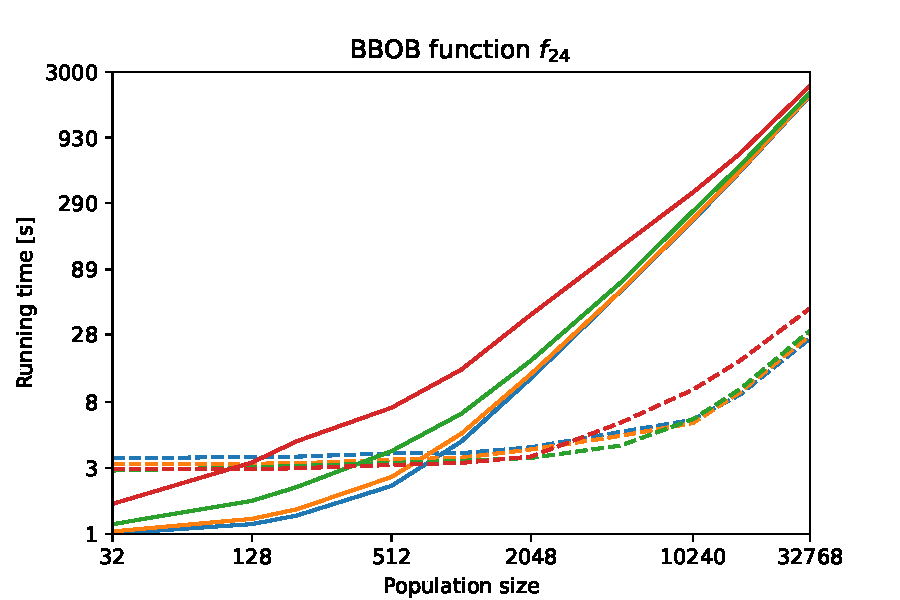
\includegraphics[width=\textwidth]{img/runs/time_pso2011_fn24_alldim.pdf}
    \end{minipage}

    \begin{minipage}{\textwidth}
        \centering
        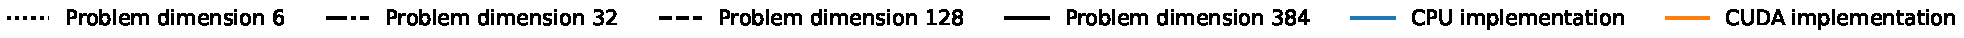
\includegraphics[width=\textwidth]{img/runs/time_pso2011_alldim_legend.pdf}
    \end{minipage}

    \caption[PSO2011 running times]{Running times of \acrlong{acc:spso2011} algorithm using problem of dimension $6$, $3$2, $128$, and $384$. The algorithm run for $1000$ generations. Populations with over $1000$ particles takes advantage of \gpu.}
\end{figure}

\begin{figure}[ht!]
    \centering
    \begin{minipage}[t]{0.32\textwidth}
        \centering
        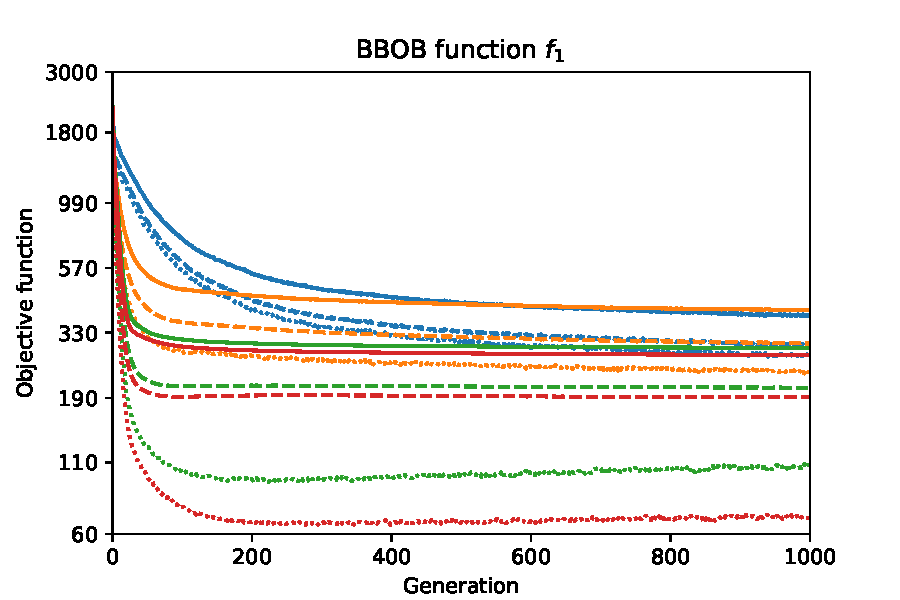
\includegraphics[width=\textwidth]{img/runs/fitness_pso2011_f1.pdf}
    \end{minipage}
    \hfill
    \begin{minipage}[t]{0.32\textwidth}
        \centering
        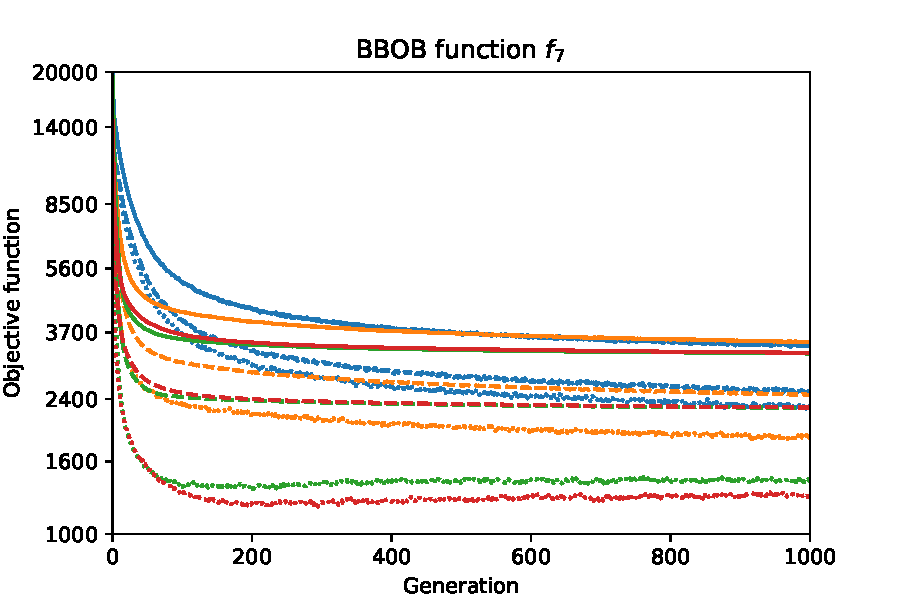
\includegraphics[width=\textwidth]{img/runs/fitness_pso2011_f7.pdf}
    \end{minipage}
    \hfill
    \begin{minipage}[t]{0.32\textwidth}
        \centering
        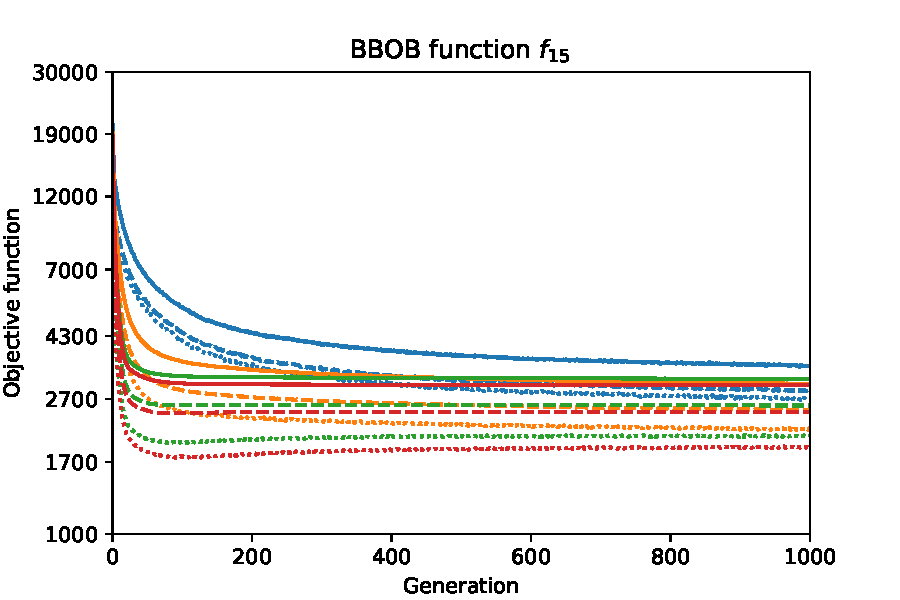
\includegraphics[width=\textwidth]{img/runs/fitness_pso2011_f15.pdf}
    \end{minipage}

    \centering
    \begin{minipage}[t]{0.32\textwidth}
        \centering
        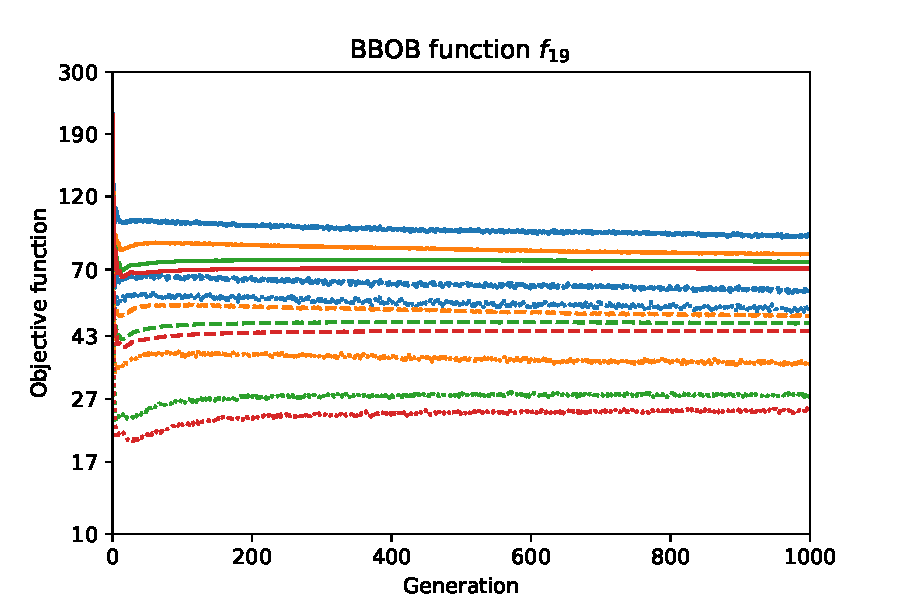
\includegraphics[width=\textwidth]{img/runs/fitness_pso2011_f19.pdf}
    \end{minipage}
    \hfill
    \begin{minipage}[t]{0.32\textwidth}
        \centering
        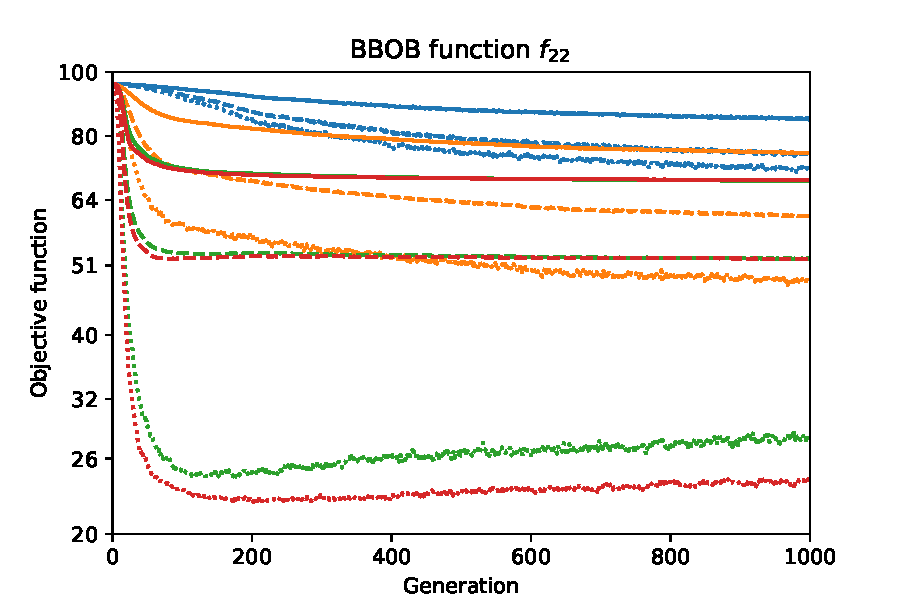
\includegraphics[width=\textwidth]{img/runs/fitness_pso2011_f22.pdf}
    \end{minipage}
    \hfill
    \begin{minipage}[t]{0.32\textwidth}
        \centering
        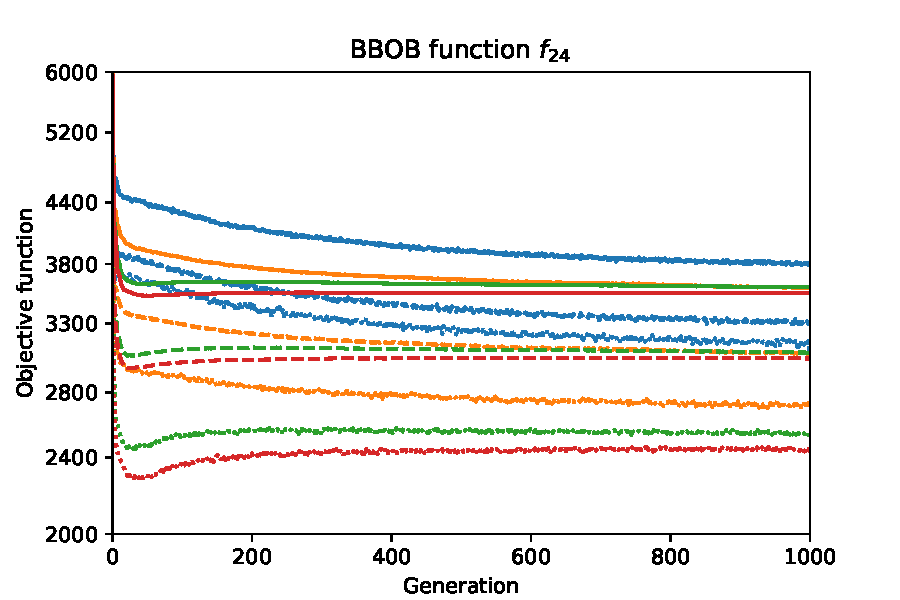
\includegraphics[width=\textwidth]{img/runs/fitness_pso2011_f24.pdf}
    \end{minipage}

    \begin{minipage}{\textwidth}
        \centering
        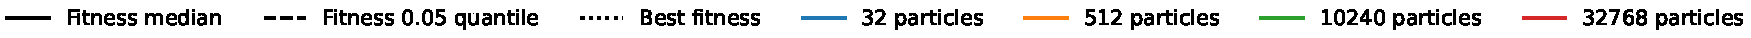
\includegraphics[width=\textwidth]{img/runs/fitness_pso2011_legend.pdf}
    \end{minipage}

    \caption[PSO2011 fitness over generations]{Median, $0.05$ quantile, and best fitness of \acrlong{acc:spso2011} algorithm using random neighborhood on problem of $128$ dimensions. I measured populations consisting of $32$, $512$, $10240$, and $32768$ particles. All the problem functions take advantage of more particles.}
\end{figure}